\section{Evaluation}
\label{sec:evaluation}

\vv{estes testes incluem o tempo de parsing? nao deveriam. deveriam só
  contar o tempo da chamada à funcao bisimilar/equivalent.}

% In this section, we analyze the performance of our algorithm
% to check the equivalence of context-free session types. 
% To do so, 
We implemented the algorithm
% we have presented thus far (sketched in
% Listings~\ref{lst:toGrammar}, \ref{lst:prune}, \ref{lst:algorithm})
in Haskell and used the Glasgow Haskell Compiler, GHC version 8.6.3,
from which we have obtained the running times we present in this
section.  Evaluation was conducted on a Mac mini equipped with a 3.6
GHz Intel Core i3, 8 GB of memory, and running MacOS 10.14.3.
%


We have tested the several combination of the previous proposals
in our algorithm on a batch of 138 tests. The results are presented 
in Figure~\ref{fig:results}.

\begin{figure}[h]
	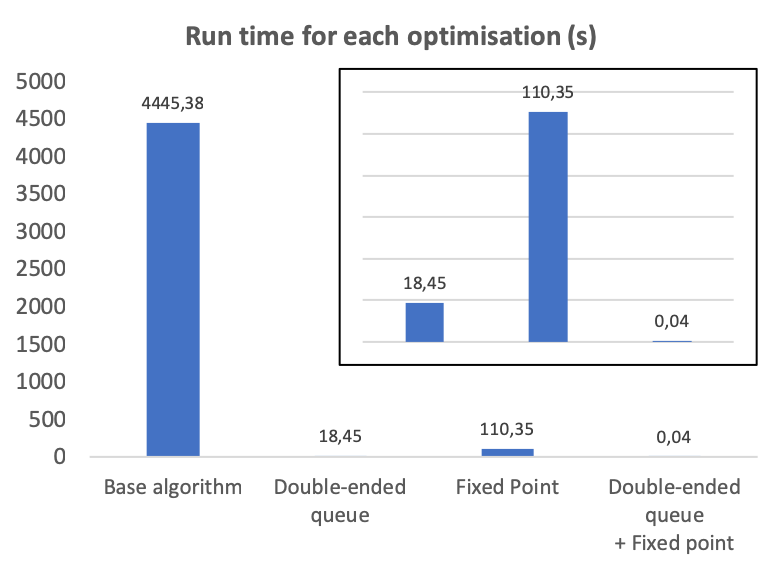
\includegraphics[height=4.8cm]{img/run_time}	\qquad 
	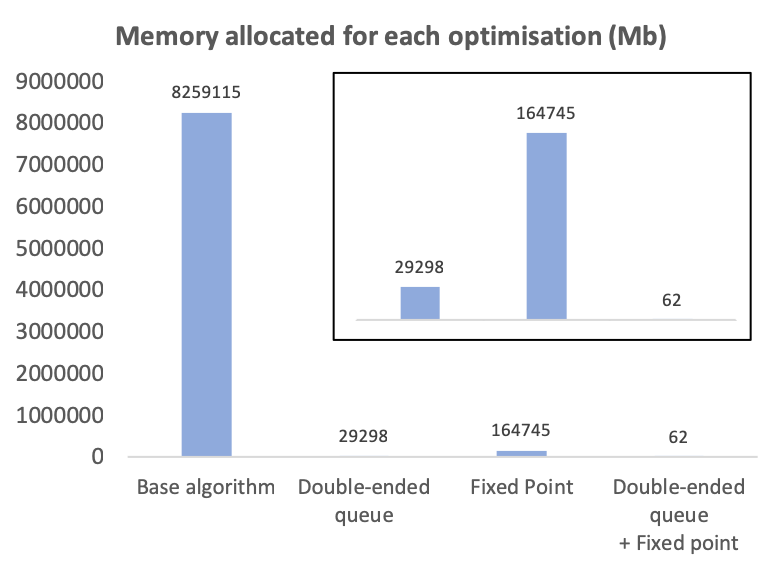
\includegraphics[height=4.8cm]{img/memory_alloc}	
	\caption{Test results: running times (on the left) and
	memory allocated (on the right) checking the equivalence 
	of context-free session types in 138 tests.}
	\label{fig:results}
\end{figure}

The running times and memory allocated are presented in
Figure~\ref{fig:results}, exhibit an improvement on more than
12,000,000\%. The running time of example in~\eqref{ex:chaotic} was
brought down to 0.008 seconds \vv{talvez seja ainda menos. as
  centesimas parecem ser a resolucao maxima do haskell; que tal correr
  o mesmo teste 100 vezes e dividir por 100?} For this reasons, our
proposal for an algorithm to check the equivalence of context-free
session types stands on adapting the simplification stage to enable
double-ended enqueueing and the computation of a fixed point at the
simplification phase Listing~\ref{lst:enhanced} presents an enhanced
version of the simplification stage coping the new proposals.



%%% Local Variables:
%%% mode: latex
%%% TeX-master: "main"
%%% End:
